\section{Diskussion}
\label{sec:Diskussion}

\subsection{Versuchsaufbau}
Der Aufbau des Versuchs ist etwas instabil, weil sich der Laser und der Sensor höhentechnisch nicht aufeinander abstimmen lassen.
Stattdessen muss der Laser nach oben \textit{gekippt} und mit beispielsweise einem Stück Papier in der Halterung eingeklemmt werden.
Die Konstruktion ist daher anfällig für Stöße am Tisch oder der Führungsschiene selbst.

\subsection{Zuverlässigkeit der Vorhersagen und Messungen}
Die Versuchsanleitung hat einen kleinen Fehler in Gleichung (6), in der das $A_0$ fehlt. Wird dieser variable Faktor in der Ausgleichsrechnung nicht berücksichtigt,
funktioniert die komplette Rechnung nicht.
Erst ein Rückschluss über die Fourier-Transformierte $g(\xi)$ deckt diesen Fehler auf.
Das Auswerten über \texttt{curve\_fit} ist \textbf{extrem} fehleranfällig, da es viele Versuchsparameter gibt, die nicht exakt bestimmt sind.
Es \textbf{müssen} geeignete Startwerte übergeben werden, da ansonsten stark abweichende Parameterwerte gefunden werden.
Auch die Parameter wie etwa $c$ für den Dunkelstrom $I_d$ oder $x_0$ für das Intensitätsmaximum sollten nicht fest eingetragen werden, da die Covarianz ansonsten gegen
unrealistische Werte für $b$ konvergiert. Daher sind die Werte variabel gehalten, werden in der Funktion selbst aber mit Startwerten versehen. \\

Zudem ist der Dunkelstrom $I_d$ nicht genau bestimmbar, da die Wolkenlage starken Einfluss auf diese Messung hat. Der Versuch wurde zu Sommerbeginn in der Uhrzeit zwischen
14 und 17 Uhr durchgeführt und fand an einer nordseitigen Fensterfront statt.
Die Abweichungen des gemessenen Dunkelstroms $I_d = (\SI{0.7}{\micro\ampere}, \SI{0.63}{\micro\ampere}) $ mit dem errechneten $(c_1, c_2) = (\SI{0.81\pm0.01}{\micro\ampere}, \SI{0.8\pm0.1}{\micro\ampere})$
ist also auf die Wetterlage zurückzuführen und liegt mit Abweichungen von $0.75 < \sfrac{I_d}{c_i} < 0.8$ in einem sehr plausiblen Bereich.
Letztlich ist dieser Faktor nur eine Verschiebung des y-Achsen-Abschnitts und hat darüber hinaus keinen Einfluss auf die Ausgleichsrechnung beziehungsweise -kurve.
Dennoch sei erwähnt, dass die eigene Sitzposition oder das Vorbeilaufen an dem Versuch einen nennenswerten Einfluss auf den Dunkelstrom hat und ein Trend in den Messdaten sichtbar werden kann.
Von einem Umsetzen während der Messung oder einer Drehung der gesamten Führungsschiene ist daher abzuraten.
Dass die über die Ausgleichsrechnung berechneten Werte für beide Dunkelströme nahezu gleich sind und nur eine Abweichung von etwa $15-27\%$ zum Realwert aufweisen, kann als erste Bestätigung für die Eignung des verwendeten Modells aufgefasst werden -- in diesem Falle der
nicht-klassische Ansatz mit den explizit gegebenen Funktionen \eqref{eqn:I} und \eqref{eqn:doppelspalt}.

\subsection{Vergleich mit der Herstellerangabe}
Die ermittelten Spaltenbreiten weichen den Herstellerangaben kaum ab. Die relativen Messunsicherheiten sind
$(b_{par, 1}, b_{par, 2}) \approx (2.5\%, 0.6\%)$. Die Werte lassen sich nähern zu $b_{par, 1} = \SI{0.0784 \pm 0.0002}{\milli\meter} \approx \SI{0.078}{\milli\meter}$ und
$b_{par, 2} = \SI{0.147 \pm 0.001}{\milli\meter} \approx \SI{0.15}{\milli\meter}$.
Damit sind die Werte den Herstellerangaben $b_{1} = \SI{0.075}{\milli\meter}$ und $b_2 = \SI{0.15}{\milli\meter}$ hinreichend genau angenähert. Die Abweichungen sind je $\Delta b_{par, 1} \approx \SI{0.0034}{\milli\meter}$ und damit um etwa $4.5\%$ beziehungsweise $\Delta b_{par, 2} = \SI{0.003}{\milli\meter}$ mit ungefähr $2\%$.
Lediglich der Spaltabstand $s$ für den Doppelspalt hat eine nennenswerte Abweichung um den Faktor 35.7. Hier ist $s = \SI{0.021 \pm 0.003}{\milli\meter} \approx \SI{0.02}{\milli\meter}$ mit einer Unsicherheit von
$14\%$. Der Herstellerwert ist $s_H = \SI{0.75}{\milli\meter}$.
Da Faktoren wie falsches Ablesen der Daten oder unvollständige Überträge der Gleichungen in ein Python-Programm ausgeschlossen werden,
wird ein anderer, systematischer Zusammenhang vermutet.
Die Abweichungen können unter anderem durch ungeeignete Näherungen innerhalb der Theorie selbst entstehen (s. Fresnel- vs. Fraunhofer-Beugung \ref{fig:fresnelFraunhofer}). \\

\subsection{Eignung der Theorie}
Die für die Rechnung verwendete Theorie der Fraunhofer-Beugung ist nur geeignet, wenn die Abstrahlwinkel auf der Spaltebene annähernd parallel sind (s. Abb. \ref{fig:fresnelFraunhofer}).
Denkbar ist, dass der Abstand $d$ mit $\SI{626.1}{\milli\meter}$ nicht groß genug ist, um eine Annäherung über $\sin{\varphi}$ zu ermöglichen.
Der in der Versuchsanleitung empfohlene Mindestabstand von $\SI{100}{\centi\meter} - \SI{120}{\centi\meter}$ kann auf der Führungsschiene nicht realisiert werden.
Mit $d = \SI{62.6}{\centi\meter}$ ist dieser Wert um knapp die Hälfte unterschritten. Zudem wurde keine Sammellinse verwendet, um diesen Abstandsverlust zu kompensieren.



\section{Erweiterte Diskussion}
\label{sec:Erweiterte Diskussion}
Die Ausgleichsrechnung für den Doppelspalt ist mit der Funktion \texttt{curve\_fit} schwer realisierbar und unterstützt die Theorie nicht vollständig.
Hier soll diskutiert werden, welche Methoden angewendet werden und welche Ursachen die Abweichungen haben können.

\subsection{Fehlerquelle Sinus-Cardinalis aus \texttt{numpy}}
Die in \texttt{numpy} definierte Funktion für den Sinus-Cardinalis \texttt{numpy.sinc(x)} ist mathematisch als $\sfrac{\sin{\pi x}}{\pi x}$ definiert. Wird der Faktor $\pi$ nicht beachtet, sind die berechneten
Werte für $b_{par}$ um einen Faktor $\pi \approx 3$ kleiner als die Realwerte. \footnote{Dies war der Grund für die ganzzahlige Abweichung aus der ersten Version des Protokolls.}

\subsection{Einzelspalt}
Die Parameter $a$ und $b_{par, 1}$ aus \eqref{eqn:Iaus} scheinen zunächst negativ korreliert zu sein, da sie miteinander multipliziert werden. Jedoch findet sich der Parameter $b_{par, 1}$
auch in dem Term für den Sinus, wodurch die Parameter dann doch gegen optimale Werte als lokale Minima konvergieren können. Um negative Parameterwerte für die \texttt{curve\_fit}-Funktion auszuschließen, wird der optionale Parameter \texttt{bounds=(0, 15)} spezifiziert,
was die Werte auf das Intervall $[0, 15]$ einschränkt. Ohne diese Einschränkung schlägt die Funktion auch tatsächlich fehl.
In einer ersten Version dieses Protokolls stimmten die Angaben aus der Auswertung (Gl. \eqref{eqn:Iaus}) und die in Python verwendete Funktion nicht ganz überein.
Mit der nun richtigen Funktion ändert sich die Qualität der Ausgleichskurve nicht, dafür aber das errechnete $b_{par, 1}$.
Die Parameter $x_0$ und $c$ können variabel gehalten werden, da sie als additive Konstanten den Graphen nur nach oben, unten, links und rechts verschieben und somit keine
Fehlerquelle darstellen. Zudem ist mit $x_0 = \SI{11.727 \pm 0.006}{\milli\meter}$ das Intensitätsmaximum und mit $c = \SI{0.81\pm0.01}{\micro\ampere}$ der von dem gemessenen Dunkelstrom abweichende,
und damit vermutlich genauere Wert, bestimmt.

Für eine bessere Nachvollziehbarkeit sei in Abbildung \ref{fig:screen1} ein Code-Auszug gezeigt. Außerdem findet sich in der Literatur\cite{download} ein Link zum Download des Verzeichnisses mit allen notwendigen Dateien und Abbildungen.
Die Python-Dateien sind sofort ausführbar, sofern \texttt{numpy}, \texttt{scipy} und \texttt{matplotlib} für Python installiert sind. \\
Analog befinden sich in diesem Verzeichnis auch die Dateien für den Doppelspalt sowie alle Abbildungen der Parameterebenen.

\begin{figure}
    \centering
    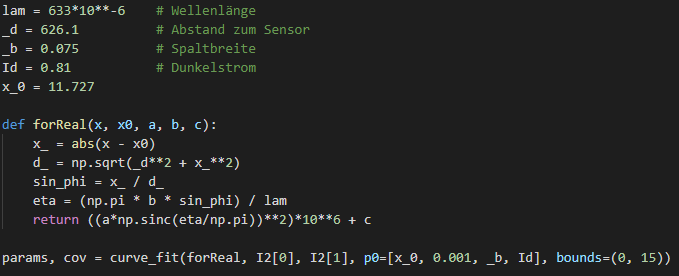
\includegraphics[width=0.9\textwidth]{plots/screen1.png}
    \caption{Code-Auszug für den Einzelspalt.}
    \label{fig:screen1}
\end{figure}

\subsection{Doppelspalt}
Die Ausgleichskurve für den Doppelspalt ist eine \textit{sehr} gute Näherung an die Messwerte. Allerdings sind die Abweichungen zu den Herstellerangaben signifikant.
Mit dem Parameterwert $s$ wird klar, dass eine oder mehrere grundlegende Annahmen oder Methoden falsch sind. Zunächst wird geprüft, ob die Spaltschablone richtig ausgerichtet und der Doppelspalt getroffen wurde,
und nicht etwa nur einer der beiden Einzelspalte. Hierfür wird für die Ausgleichsrechnung die Funktion des Einzelspalts verwendet (s. Abb. \ref{fig:doppeleinzel}).

\begin{figure}
    \centering
    \begin{subfigure}{.5\textwidth}
      \centering
      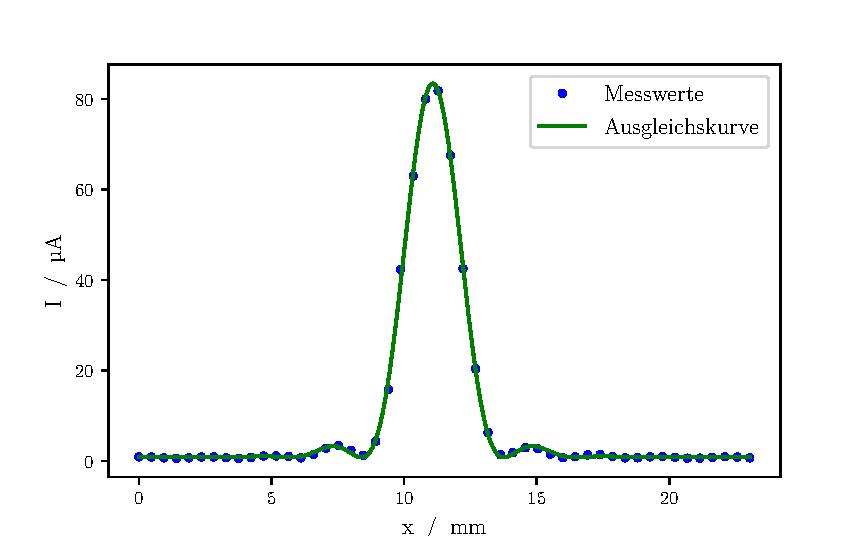
\includegraphics[width=.7\textwidth]{python/DoppelspaltFit.pdf}
      \caption{Ausgleichskurve mit Doppelspaltfunktion.}
    \end{subfigure}%
    \begin{subfigure}{.5\textwidth}
        \centering
      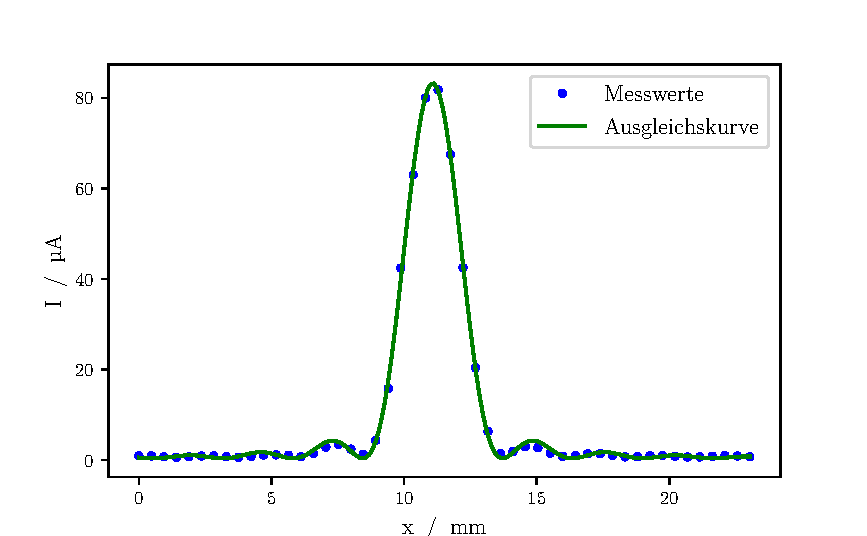
\includegraphics[width=.7\linewidth]{python/DoppelspaltFitEinzel.pdf}
      \caption{Ausgleichskurve mit Einzelspaltfunktion.}
    \end{subfigure}
      \caption{Ausgleichskurven für den Doppelspalt.}
      \label{fig:doppeleinzel}
\end{figure}

Die Einzelspaltfunktion eignet sich der Abbildung nach ebenfalls für eine Ausgleichsrechnung, ist qualitativ jedoch etwas schlechter. Bei genauer Betrachtung liegen die Extremstellen nicht genau übereinaner.
Die errechneten Parameterwerte sind aber sehr ähnlich. Der Wert der Einzelspaltfunktion $b_{par, 2e} = \SI{0.1504 \pm 0.0008}{\milli\meter}$ ist dem der Doppelspaltfunktion $b_{par, 2} = \SI{0.147 \pm 0.001}{\milli\meter}$ kaum verschieden,
und der Dunkelstrom $c_{par, 2e} = \SI{0.4 \pm 0.1}{\micro\ampere}$ ist im Vergleich zu dem real gemessenen Wert von $\SI{0.63}{\micro\ampere}$ ebenfalls in einem sinnvollen Bereich.
Der Parameter $s$ wird in dieser Rechnung nicht berücksichtigt.

\begin{table}
    \centering
    \caption{Parameterwerte des Doppelspalts mit der Einzelspaltfunktion.}
    \label{tab:parDoppelEinzel}
    \begin{tabular}{c S[table-format=1.5]@{\,\( \pm \)\,}S[table-format=1.5] 
        S[table-format=1.4]@{\,\( \pm \)\,}S[table-format=1.4] 
        S[table-format=1.1]@{\,\( \pm \)\,}S[table-format=1.1]
        S[table-format=1.3]@{\,\( \pm \)\,}S[table-format=1.3]}
        \toprule
        & \multicolumn{2}{c}{$a$} & \multicolumn{2}{c}{$b_{par, 1}\:/\:\si{\milli\meter}$} & \multicolumn{2}{c}{$c\:/\:\si{\micro\ampere}$} & \multicolumn{2}{c}{$x_0\:/\:\si{\milli\meter}$} \\
        \midrule
        Doppelspalt & 0.00910&0.00003 & 0.1504&0.0008 & 0.38&0.1 & 11.078&0.006\\
    \end{tabular}
\end{table}

Die Funktion für den Einzelspalt ist in \ref{fig:screen1} abgebildet. Die für den Doppelspalt in Abbildung \ref{fig:screen2}.

\begin{figure}
    \centering
    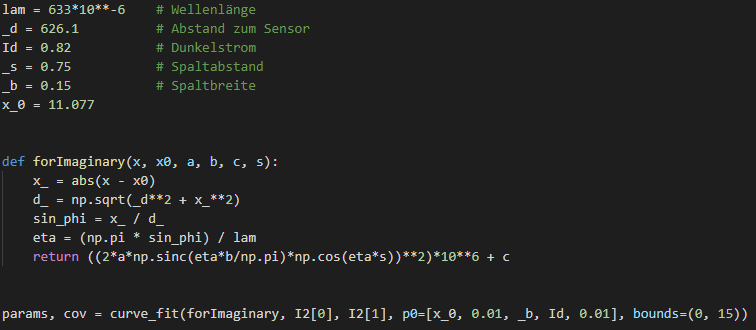
\includegraphics[width=0.9\textwidth]{plots/screen2.png}
    \caption{Code-Auszug für den Doppelspalt.}
    \label{fig:screen2}
\end{figure}

Dass nur ein Einzelspalt gemessen wurde, wird an dieser Stelle aber ausgeschlossen. Zwar ist der Wert für $b_2$ sehr gut genähert, jedoch ist der Dunkelstrom nur halb so groß wie beim Einzelspalts.
Da mit der Doppelspaltfunktion aber der gleiche Wert $c \approx \SI{0.8}{\micro\ampere}$ wie für den Einzelspalt berechnet wird, ist dieser Wert wahrscheinlich auch der Realwert.
Außerdem ist die Qualität der Ausgleichskurve wie bereits erwähnt sichtlich besser. 

\subsubsection{Spaltabstand}
Der Spaltabstand $s$ ist eine Größe, die nur den Doppelspalt betrifft. Trotz der qualitativ hochwertigen Ausgleichskurve ist der ermittelte Wert für $s$ mit einem Faktor
von etwa 35.7 eine derart große Abweichung, dass die Theorie geprüft werden muss.
Genau genommen können die wahrscheinlichsten Ursachen wie folgt zusammengefasst werden.
\begin{enumerate}
    \item Systematische Messfehler
    \item Eignung der Theorie
    \item Methodik der Ausgleichsrechnung
\end{enumerate}
\textbf{Systematische Fehler}, die in der Sensorik liegen oder dem Aufbau geschuldet sind, können nicht ausgeschlossen, nachträglich aber auch nicht geprüft werden.

Die \textbf{Eignung der Theorie} ist bereits thematisiert worden. Von Bedeutung sind in diesem Falle ungeeignete Näherungen, die nicht gemacht werden dürfen, weil der Versuchsaufbau nicht
den Anforderungen entspricht. Denkbar sind in diesem Zusammenhang auch nicht beachtete Störfunktionen, die in der Theorie nicht behandelt werden.

\subsection{Parameterebene und Ausgleichsrechnung}
Im weiteren Verlauf wird die Methodik der Ausgleichsrechnung diskutiert.
Wie bereits in der Auswertung erklärt, sucht die Methode der kleinsten Quadrate nach Minima auf sogenannten Parameterebenen beziehungsweise -räumen.
Die Auswertung stellt in den Abbildungen \ref{fig:ls1} bis \ref{fig:lsd3s} die Parameterebenen gegenüber, sodass Minima geometrisch dargestellt und abgelesen werden können.
Der grundlegende Gedanke ist, dass sich kleinere, lokale Minima um das globale Minimum verteilen können.
Letztlich ist dies auch der Grund, warum die Funktion \texttt{curve\_fit} mit Startwerten versehen werden muss, da die Funktion nicht beliebig große Intervalle der Parameter durchläuft und als Ergebnis nur ein lokales Minimun in der Startwertumgebung findet.
So ein globales Verhalten ist auch nicht immer sinnvoll, da gesuchte Parameter oftmals einen Erwartungswert besitzen -- etwa wie hier die Spaltbreite $b$.
In den Abbildungen kann beobachtet werden, dass alle Parameterwerte gegen ein bestimmtes Wertepaar konvergieren. In der Umgebung des Minimums gibt es auch keine weiteren Minima. Zudem ist die Umgebung um den Punkt $(a_0, b_0)$ streng monoton fallend.
Hiermit wird ausgeschlossen, dass es ein zweit- oder drittbestes Optimum gibt.
Die Kurvenschar des Einzelspalts \ref{fig:2d} unterstreicht das konvergente Verhalten der Parameter und zeigt keine Anomalien für oder um den Realwert $b = 0.075$.\\

Die Darstellung des Doppelspalts ist wie in der Auswertung bereits erwähnt schwieriger, da die Geometrie eine Dimension höher ist.
Die hier verwendete Methode -- um die Abhängigkeit dennoch geometrisch darzustellen -- ist die Gegenüberstellung von verschiedenen Parameterebenen mit unterschiedlichen Werten für $s$.
Sinnvoll ist eine Betrachtung der Ebene für den Realwert von $s$ und für das errechnete Optimum von $s$.
Ein Vergleich der beiden Ebenen, welche je einmal große und einmal kleine Intervalle für $(a, b)$ besitzen, zeigt, dass das Verhalten der Konvergenz gleich bleibt. Das Minimum verschiebt sich nur minimal, wird aber bedeutend kleiner für $s \approx 0.022$. Auch hier finden sich keine Anomalien in der Umgebung des Realwertes für $s$.\\

Letztlich sind noch zwei nicht optimale Ausgleichskurven für die Realwerte von $b$ und $s$ den optimalen Kurven in den Abbildungen \ref{fig:ggn1} und \ref{fig:ggn2} gegenübergestellt.
Dort ist sichtbar, dass die realen Spaltbreiten beziehungsweise -abstände keine passenden Kurven erzeugen. \\

Es gibt drei Voraussetzungen für die Methode der kleinsten Quadrate, die hier auch alle erfüllt sind.
\begin{enumerate}
    \item Es liegen wesentlich mehr Messdaten als Parameterwerte vor.
    \item Die Messwerte sind normalverteilt.
    \item Das verwendete Modell beschreibt das Verhalten der Messwerte.
\end{enumerate}

\subsubsection{Tool zum Testen des Beugungsmusters}
Es gibt ein Online-Tool, mit dem über verschiedene Slider die Form der Beugungsfigur in Abhängigkeit seiner Parameter verändert werden kann.
Dies ist besonders hilfreich, um zu verstehen, dass es für jede Figur nur einen Parametervektor $\vec{\beta}$ geben kann, der die Messwerte genau approximiert.\\
\textbf{Einzelspalt:} \url{https://www.leifiphysik.de/optik/beugung-und-interferenz/grundwissen/einzelspalt}\\
\textbf{Doppelspalt:} \url{https://www.leifiphysik.de/optik/beugung-und-interferenz/grundwissen/doppelspalt}

\subsection{Fazit}
Der Versuch ist hinreichend durchführbar und die Ergebnisse bestätigen den Wellencharakter des Lichts (\textit{Interferenzmuster}).
Trotz der varianten Wolkenlage sind die Messwerte um das Intensitätsmaximum symmetrisch verteilt.
Lediglich die Rahmenbedingungen des Aufbaus sind genau zu bestimmen und an manchen Stellen anzupassen, wie etwa der Maximalabstand $d$. Die Form der gemessenen Beugungsfigur selbst besitzt jedoch keine sichtbaren Anomalien.
Vernünftige Stative für den Laser wären eine nennenswerte Verbesserung. Außerdem würde eine Sammellinse wesentlich stabilere Messungen ermöglichen. Damit könnten auch ungeeignete Näherungen innerhalb der Theorie ausgeschlossen werden.
Die Auswertung der Parameterebenen schließt ebenfalls unerwünschte Anomalien aus, die die Punkt-erzeugende \texttt{curve\_fit}-Funktion sonst ignoriert. 
Zum Schluss sei erwähnt, dass eine Schutzklappe beziehungsweise -vorrichtung für den Laser, oder ausdrückliche Sicherheitshinweise ratsam sind, da der Laser vorheizen muss und nicht sofort absehbar ist, ob der Laser eingeschaltet
ist beziehungsweise funktioniert.